% !TeX program = pdflatex
% ============================================================
% CiboAmico — Relazione finale ISPW (Tor Vergata, A.A. 2025/2026)
% Prof. Davide Falessi & Prof. Guglielmo De Angelis
% Versione in ITALIANO
% ============================================================
\documentclass[12pt,a4paper,oneside]{report}

% --- Lingua e codifica ---
\usepackage[italian]{babel}
\usepackage[utf8]{inputenc}
\usepackage[T1]{fontenc}
\usepackage{microtype}

% --- Geometria e tipografia ---
\usepackage[margin=2.5cm]{geometry}
\usepackage{setspace}
\onehalfspacing

% --- Immagini, tabelle ---
\usepackage{graphicx}
\usepackage{booktabs}
\usepackage{colortbl}
\usepackage{float}
\usepackage{pdflscape}
\usepackage{array}
\usepackage{multirow}
\usepackage{caption}
\captionsetup{font=small,labelfont=bf}

% --- Elenchi e simboli ---
\usepackage{enumitem}
\usepackage{csquotes}
\usepackage{amsmath,amssymb}
\usepackage{xcolor}

% --- UML / diagrammi ---
\usepackage{tikz}
\usetikzlibrary{shapes,shapes.geometric,positioning,arrows.meta}

% --- Codice Java ---
\usepackage{listings}
\definecolor{codegray}{RGB}{245,245,245}
\definecolor{codekeyword}{RGB}{0,0,204}
\definecolor{codecomment}{RGB}{0,128,0}
\definecolor{codestring}{RGB}{163,21,21}
\lstset{
    language=Java,
    basicstyle=\ttfamily\footnotesize,
    keywordstyle=\color{codekeyword},
    commentstyle=\color{codecomment},
    stringstyle=\color{codestring},
    backgroundcolor=\color{codegray},
    frame=single,
    breaklines=true,
    columns=fullflexible,
    captionpos=b
}

% --- Collegamenti ---
\usepackage{hyperref}
\hypersetup{
    colorlinks=true,
    linkcolor=black,
    urlcolor=blue,
    citecolor=black
}

% ============================================================
\begin{document}

% --- Frontespizio ---
\begin{titlepage}
    \centering
    \large
    \textbf{UNIVERSITÀ DEGLI STUDI DI ROMA ``TOR VERGATA''} \\[0.3cm]
    \large Macroarea di Ingegneria \\
    Dipartimento di Ingegneria Civile e Ingegneria Informatica (DICII) \\[1.2cm]

    \scshape\Large Corso di Laurea in Ingegneria Informatica \\[0.3cm]
    \large Ingegneria del Software e Progettazione Web (ISPW) \\[1.5cm]

    \rule{\linewidth}{0.4mm} \\[0.4cm]
    {\huge\bfseries CiboAmico} \\[0.3cm]
    \large\itshape Piattaforma per la gestione del cibo in casa, la riduzione degli sprechi e l'ottimizzazione della spesa \\
    \rule{\linewidth}{0.4mm} \\[1.5cm]

    \begin{minipage}{0.5\textwidth}
        \begin{flushleft} \large
            \emph{Docenti:} \\
            Prof. Davide Falessi \\
            Prof. Guglielmo De Angelis
        \end{flushleft}
    \end{minipage}
    \hfill
    \begin{minipage}{0.42\textwidth}
        \begin{flushright} \large
            \emph{Autore:} \\
            \textbf{Michele \textsc{Damiano}} \\
            Matricola: 0324516 \\
            \href{mailto:michele.damiano@students.uniroma2.eu}{\small michele.damiano@students.uniroma2.eu}
        \end{flushright}
    \end{minipage} \\[2.5cm]

    \vfill
    {\large Anno Accademico 2025/2026} \\[0.2cm]
    {\large Data di consegna: \today}
\end{titlepage}

% --- Abstract / Sommario ---
\chapter*{Sommario}
\markboth{Sommario}{}
\addcontentsline{toc}{chapter}{Sommario}

CiboAmico risolve il problema dello spreco alimentare domestico e della frammentazione del commercio a chilometro zero. La piattaforma offre una gestione intelligente della dispensa, un motore di matching delle ricette con sostituzione automatica degli ingredienti e un marketplace locale per l'interazione diretta tra clienti, commercianti e amministratori. L'architettura software si basa sul pattern \emph{Boundary-Control-Entity} (BCE). Ho implementato una doppia interfaccia utente intercambiabile a runtime---un'interfaccia grafica in JavaFX e una riga di comando (CLI)---orchestrata tramite una \texttt{ViewFactory} e disaccoppiata dai controller applicativi stateless mediante l'uso di Bean (DTO).

Per la persistenza ho progettato tre modalità (JDBC MySQL, File System JSON e Demo in-memory) gestite da un'Abstract Factory di DAO. Ho inoltre applicato diversi pattern GoF, tra cui \emph{Strategy} per la logica di matching, \emph{Facade}, \emph{Observer} per la gestione degli ordini, \emph{Singleton} e due \emph{Adapter} per OpenFoodFacts e JakartaMail, garantendo la sicurezza delle credenziali tramite hashing SHA-256 e salt. La correttezza e la qualità della logica di business sono verificate da 92 unit test JUnit 5, con una Line Coverage dell'81.4\%, e dall'assenza di violazioni rilevate su SonarCloud.

\newpage

% --- Indice ---
\tableofcontents
\newpage

% ============================================================
% CAPITOLI
% ============================================================
% ============================================================
% CAPITOLO 1 — SPECIFICHE DEI REQUISITI SOFTWARE (SRS)
% ============================================================
\chapter{Specifiche dei Requisiti Software}
\label{cap:srs}

% ------------------------------------------------------------
\section{Introduzione}
\label{sec:intro}

\subsection{Scopo del documento}
\label{subsec:scopo}

Questo documento definisce i requisiti software di \textbf{CiboAmico}, il progetto finale del corso ISPW (Università di Roma ``Tor Vergata'', A.A.\ 2025/2026, Prof. Davide Falessi, Prof. Guglielmo De Angelis).

Lo scopo è fissare cosa il sistema deve fare in modo chiaro e verificabile, lasciando campo alla progettazione e ai test. Il documento serve sia a chi sviluppa, per tenere fede all'architettura Boundary-Control-Entity (BCE), sia a chi valuta il prodotto, per confrontare i flussi funzionali con le richieste iniziali.

\subsection{Panoramica del sistema}
\label{subsec:panoramica}

CiboAmico è un'applicazione desktop JavaFX che aiuta a gestire il cibo in casa, evitare sprechi e ottimizzare la spesa, collegando l'utente ai commercianti di prossimità. Il sistema segue il pattern Boundary-Control-Entity (BCE) e coinvolge quattro attori: Cliente, Venditore, Nutrizionista e Amministratore. Due sistemi esterni sono raggiunti tramite Adapter: OpenFoodFacts (lettura dei dati nutrizionali dal codice a barre) e JakartaMail (invio di notifiche). La persistenza è intercambiabile a runtime tra una modalità \textit{Demo} (in-memory) e una \textit{Full} (MySQL via JDBC).

Il sistema ha tre aree funzionali:
\begin{itemize}
    \item \textbf{Dispensa}: il Cliente traccia i prodotti in casa, vede le scadenze e viene avvisato prima che il cibo si deteriori;
    \item \textbf{Ricette}: il sistema propone ricette compatibili con gli ingredienti disponibili, sostituendo quelli mancanti;
    \item \textbf{Marketplace}: i Venditori pubblicano i prodotti, i Clienti fanno ordini diretti (un compratore, un venditore) e l'Amministratore approva venditori e ricette.
\end{itemize}

\subsection{Requisiti hardware e software}
\label{subsec:requisiti_hw_sw}

L'applicazione è cross-platform grazie alla JVM. I requisiti minimi sono: processore dual-core a 64-bit, 2~GB di RAM, 150~MB di disco e schermo $1024\times768$. In modalità JDBC, che esegue anche il server MySQL locale, si consigliano 4~GB di RAM, 500~MB su SSD e una scheda grafica compatibile con OpenGL 2.0.

A livello software servono: OpenJDK 17 LTS, JavaFX 17+, Maven 3.9+ e, per la modalità database, MySQL 8.0+. Per sviluppo e controllo qualità si usano IntelliJ IDEA (con EclEmma per la coverage), JUnit 5, SonarCloud e GitHub Actions. I diagrammi UML sono realizzati con StarUML o Draw.io.

\subsection{Sistemi correlati, pro e contro}
\label{subsec:relazionati}

Di seguito due sistemi esistenti che coprono solo in parte quello che fa CiboAmico.

\paragraph{Too Good To Go}
Piattaforma B2C per il recupero delle eccedenze alimentari: connette l'utente con commercianti e supermercati locali.
\begin{itemize}
    \item \textbf{Pro}: rete capillare di partner con offerte geolocalizzate in tempo reale; riduce attivamente lo spreco commerciale offrendo cibo a prezzi ridotti.
    \item \textbf{Contro}: non traccia la dispensa di casa, quindi dopo l'acquisto non aiuta a gestire le scadenze; l'acquisto è una \emph{Magic Box} a sorpresa, non si scelgono i singoli prodotti né si pianificano ricette o diete.
\end{itemize}

\paragraph{SuperCook}
Motore di ricerca di ricette in base agli ingredienti già in dispensa.
\begin{itemize}
    \item \textbf{Pro}: matching potente che trova subito molte ricette a partire dagli ingredienti inseriti; ampio database con filtri per tipo di piatto e intolleranze.
    \item \textbf{Contro}: non ha un canale di acquisto integrato, quindi per gli ingredienti mancanti bisogna provvedere da soli; non sostituisce automaticamente gli ingredienti, escludendo ricette realizzabili con piccole variazioni.
\end{itemize}

\paragraph{Posizionamento di CiboAmico}
CiboAmico unisce i due approcci: gestisce la dispensa contro lo spreco (come SuperCook), propone ricette con sostituzioni intelligenti e, se manca qualcosa, permette di comprarlo dai produttori locali a chilometro zero (come Too Good To Go), tutto in una sola applicazione.

% ------------------------------------------------------------
\section{User Stories}
\label{sec:user_stories}

\begin{enumerate}
    \item \textbf{US-1}: Come Cliente, voglio ricevere notifiche preventive sulle date di scadenza dei prodotti presenti nella mia dispensa, in modo che possa consumare gli alimenti in tempo ed evitare lo spreco di cibo.
    \item \textbf{US-2}: Come Cliente, voglio visualizzare le ricette compatibili con gli ingredienti disponibili in dispensa, in modo che possa cucinare senza dover effettuare nuovi acquisti.
    \item \textbf{US-3}: Come Cliente, voglio ordinare un prodotto direttamente da un venditore locale, in modo che possa ricevere cibo fresco proveniente dal mio territorio.
\end{enumerate}

% ------------------------------------------------------------
\section{Requisiti Funzionali}
\label{sec:requisiti_funzionali}

\begin{enumerate}
    \item \textbf{RF-1}: Il sistema deve confrontare quotidianamente le date di scadenza degli alimenti nella dispensa con la data corrente, inviando un avviso al cliente per ogni prodotto la cui scadenza sia entro tre giorni.
    \item \textbf{RF-2}: Il sistema deve suggerire al cliente un elenco di ricette in cui gli ingredienti richiesti siano un sottoinsieme degli ingredienti non scaduti presenti nella dispensa.
    \item \textbf{RF-3}: Il sistema deve registrare una nuova transazione di acquisto associando il cliente al venditore e decrementando la scorta del prodotto in misura pari alla quantità ordinata.
\end{enumerate}

\subsection{Glossario dei Termini di Dominio}
\begin{description}
    \item[\textbf{Dispensa}]: rappresentazione digitale degli alimenti presenti nell'inventario domestico dell'utente, con quantità e date di scadenza.
    \item[\textbf{Ricetta compatibile}]: ricetta i cui ingredienti richiesti sono presenti, oppure sostituibili in modo equivalente, nella dispensa dell'utente.
    \item[\textbf{Ordine diretto}]: transazione che associa un singolo cliente acquirente a un unico venditore, senza passare da un carrello condiviso o intermediari.
    \item[\textbf{Disponibilità del prodotto}]: quantità di un prodotto attualmente vendibile, che non può mai essere negativa e viene aggiornata dopo ogni acquisto.
\end{description}

% ------------------------------------------------------------
\section{Use Cases}
\label{sec:use_cases}

\subsection{Diagramma dei casi d'uso}
\label{subsec:uc_diagramma}

\begin{figure}[H]
    \centering
    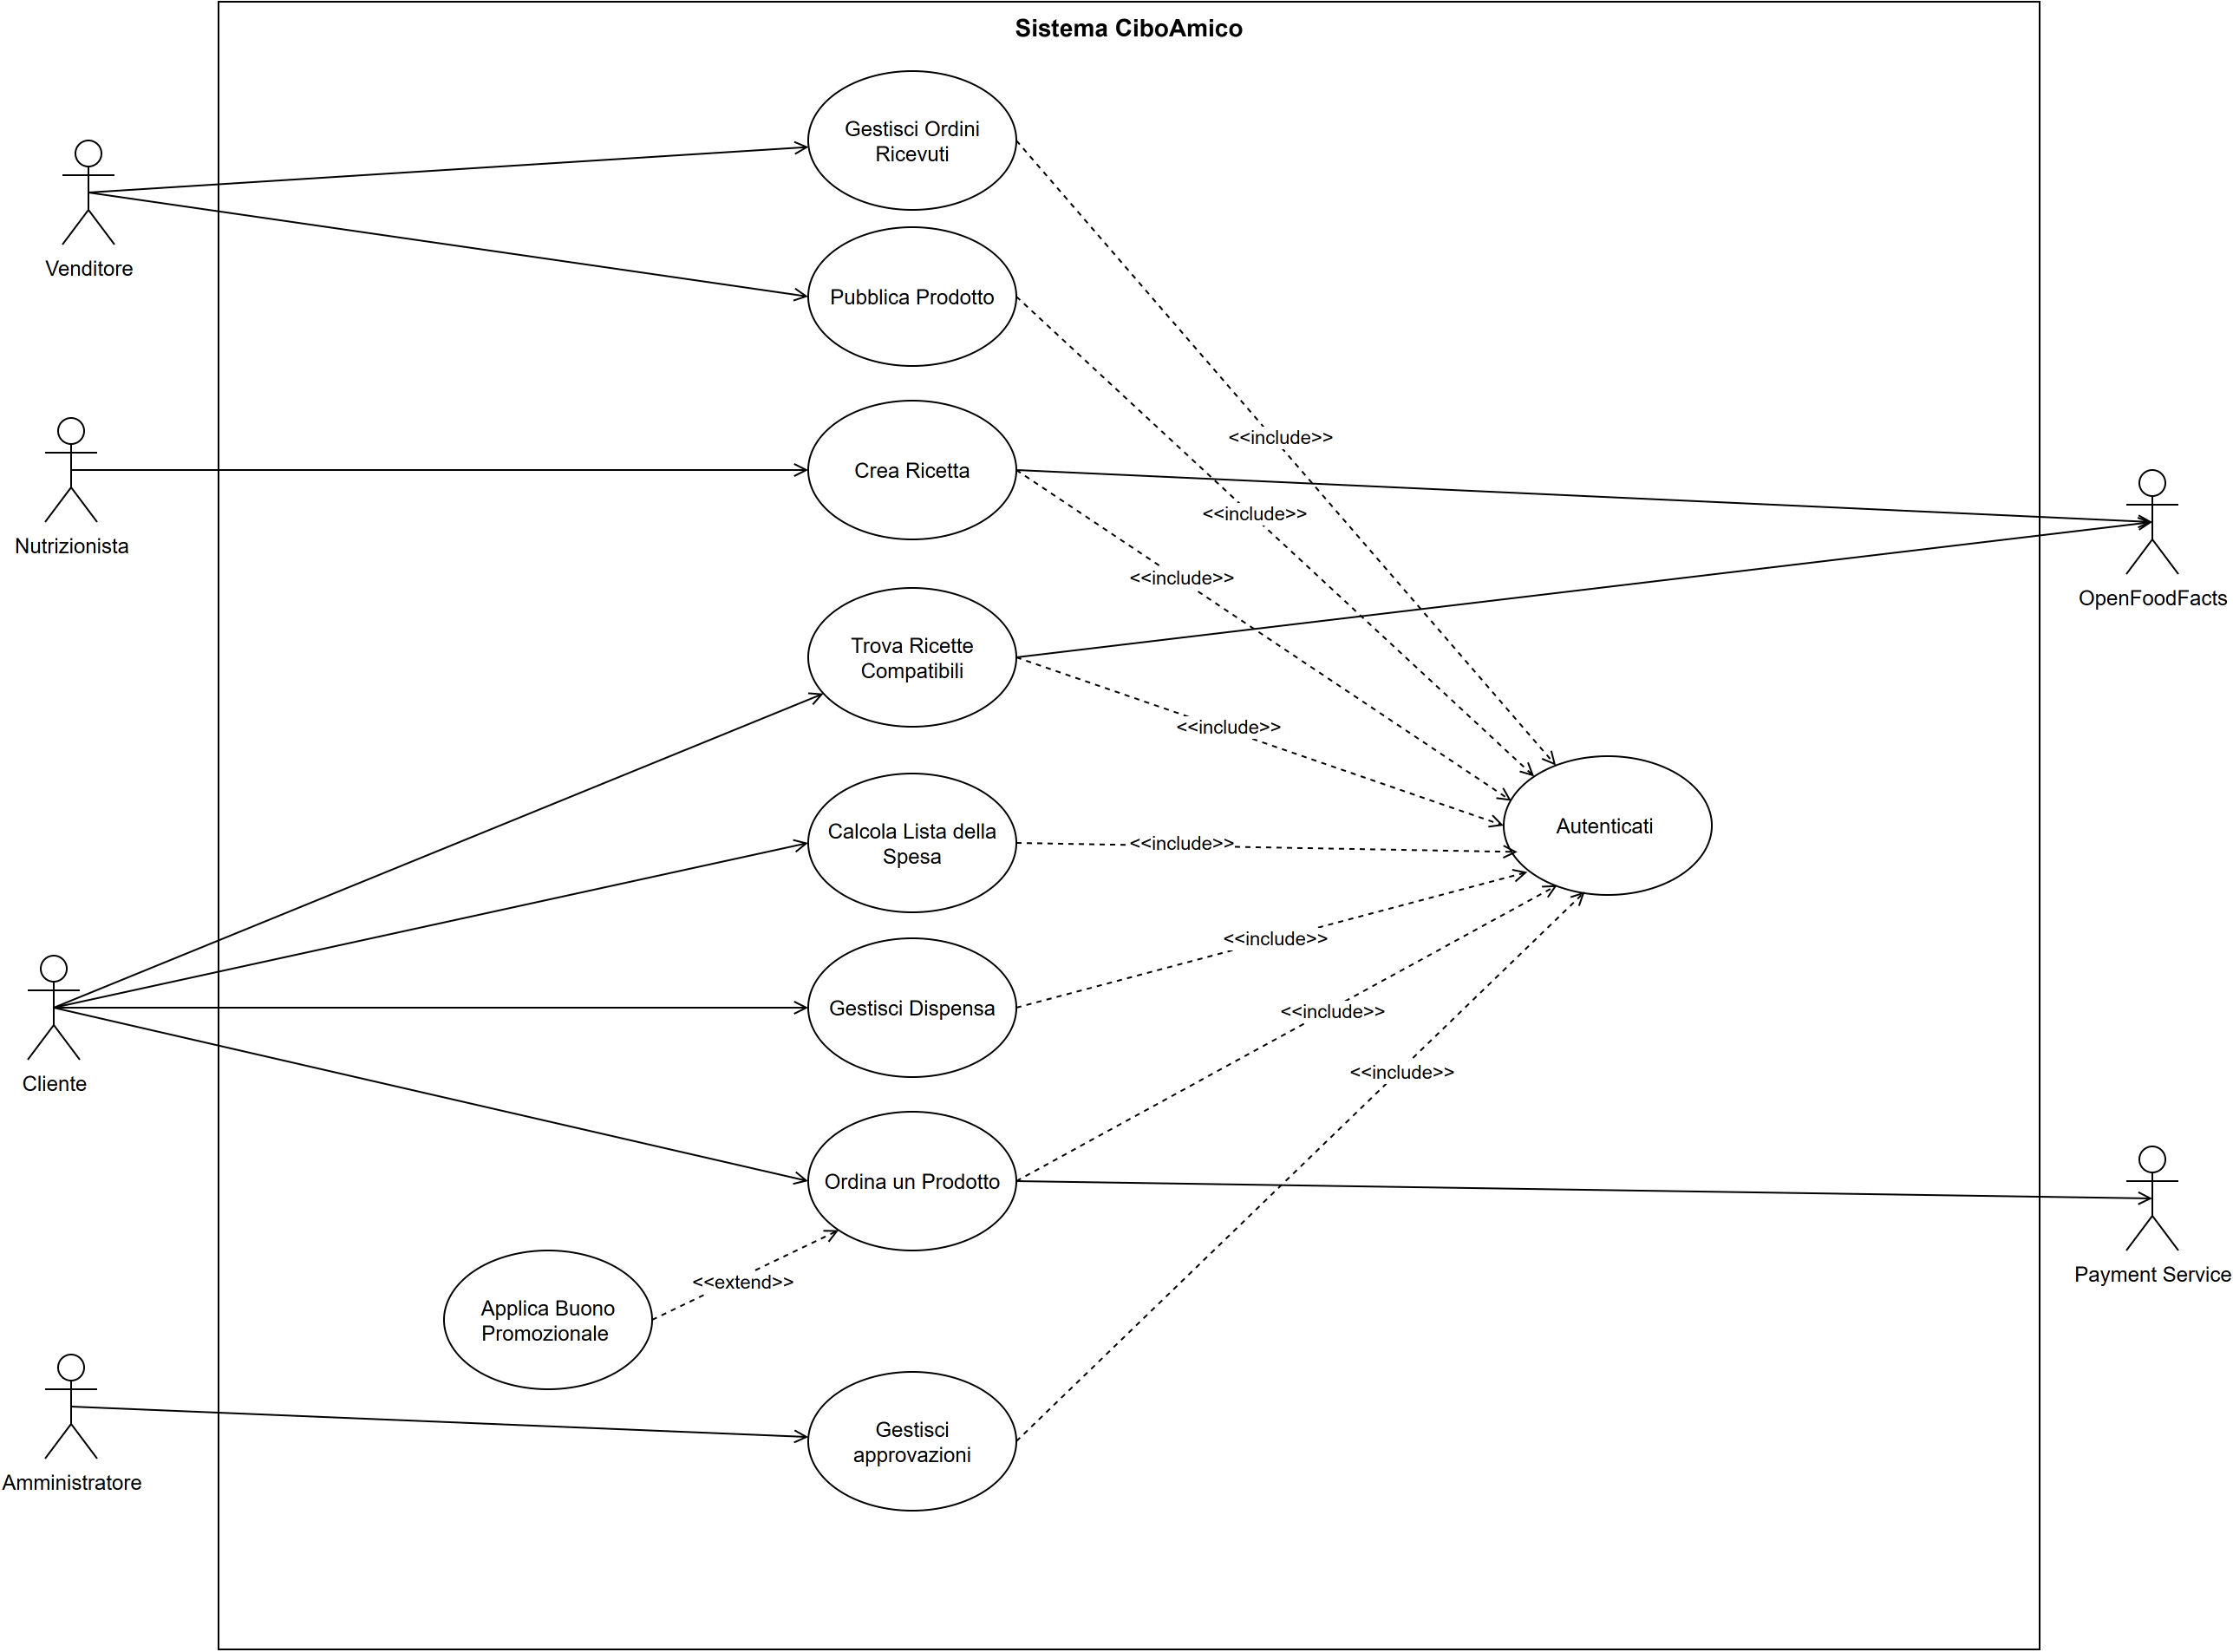
\includegraphics[width=0.95\textwidth]{figures/usecase_diagram_hr.png}
    \label{fig:usecase_diagram}
\end{figure}

Il caso d'uso \textbf{Ordina un Prodotto} è stato progettato con un grado di astrazione che consente di modellare funzionalità distinte. In questa implementazione, il caso d'uso secondario \textbf{Applica Buono Promozionale} è associato al caso d'uso primario tramite una relazione di \emph{extend}: l'attore Cliente può utilizzare questa funzionalità estesa solo se si autentica correttamente nel sistema (relazione di \emph{include} verso \textbf{Autenticati}) e proseguendo poi il flusso del caso d'uso \textbf{Ordina un Prodotto}. Analogamente, \textbf{Autenticati} è incluso da più casi d'uso, a sottolinearne il riuso nell'ambito delle funzionalità principali.

\subsection{Internal Steps}
\label{subsec:uc_internal_steps}

\subsubsection{Ordina un Prodotto}
\label{u:uc04}

\textbf{Scenario principale:}
\begin{enumerate}
    \item Il Sistema individua i prodotti disponibili sul marketplace con prezzi, scorte residue e venditori.
    \item Il Cliente richiede di aggiungere un prodotto all'ordine, indicandone la quantità desiderata.
    \item Il Sistema convalida che la quantità richiesta non superi la scorta residua del prodotto.
    \item Il Sistema calcola l'importo totale della transazione. \label{step:calcolo_totale}
    \item Il Cliente richiede di confermare l'acquisto. \label{step:conferma_acquisto}
    \item Il Sistema richiede al Payment Service l'autorizzazione all'addebito per l'importo calcolato.
    \item Il Sistema registra l'ordine in attesa di approvazione e decrementa la scorta residua dei prodotti ordinati.
    \item Il Sistema invia una notifica al Venditore per segnalare l'ordine ricevuto.
\end{enumerate}

\textbf{Estensioni:}
\begin{itemize}
    \item \textbf{3a. Superamento della scorta residua:}
    \begin{enumerate}
        \item Il Sistema rileva che la quantità inserita dal Cliente è superiore alla disponibilità corrente del prodotto.
        \item Il Sistema segnala l'anomalia al Cliente indicando la massima quantità acquistabile.
        \item Il flusso di controllo ritorna al passo 2.
    \end{enumerate}
    \item \textbf{4a. Richiesta di applicazione di un buono promozionale (tramite l'estensione del caso d'uso Applica Buono Promozionale):}
    \begin{enumerate}
        \item Il Cliente richiede di applicare un codice di buono promozionale all'ordine corrente.
        \item Il Sistema convalida la validità temporale del buono promozionale e la sua associazione con il Venditore del prodotto selezionato.
        \item Il Sistema ricalcola l'importo totale della transazione applicando lo sconto previsto dal buono promozionale.
        \item Il flusso di controllo prosegue dal passo 5 dello scenario principale.
    \end{enumerate}
    \item \textbf{6a. Autorizzazione di pagamento negata:}
    \begin{enumerate}
        \item Il Sistema riceve l'esito negativo dall'autorizzazione del Payment Service.
        \item Il Sistema segnala al Cliente il fallimento del pagamento.
        \item Il flusso di controllo ritorna al passo 5.
    \end{enumerate}
\end{itemize}


% CAPITOLO 2 — STORYBOARDS
\chapter{Storyboards}
\label{cap:storyboards}

\section{Autenticazione e Area Personale}

\subsection{Autenticati}
La schermata di accesso permette all'utente di autenticarsi inserendo le proprie credenziali (email e password).
\begin{figure}[H]
    \centering
    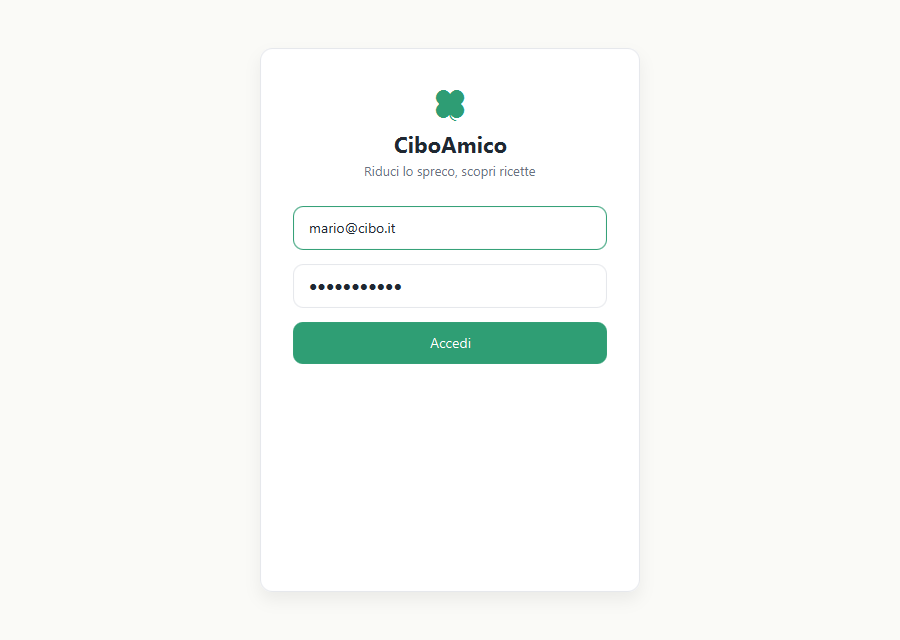
\includegraphics[width=0.8\textwidth]{figures/schermata-login.png}
    \caption{Schermata di autenticazione al sistema.}
    \label{fig:sb_login}
\end{figure}

\subsection{Home (Cliente)}
Completata l'autenticazione, il Cliente raggiunge la dashboard principale, dalla quale accede alle aree del sistema.
\begin{figure}[H]
    \centering
    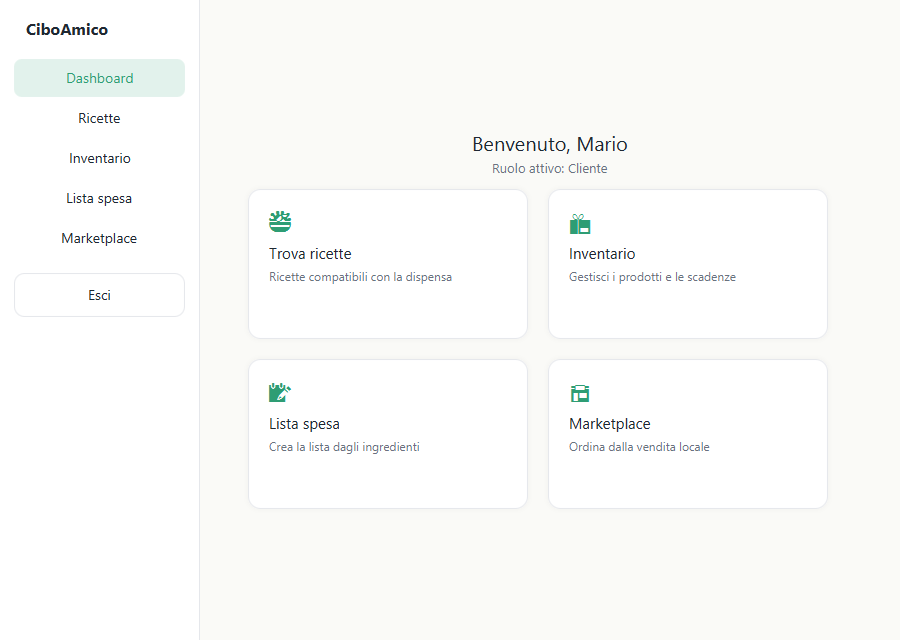
\includegraphics[width=0.8\textwidth]{figures/schermata-home.png}
    \caption{Dashboard principale lato Cliente.}
    \label{fig:sb_home}
\end{figure}

\section{Gestione Domestica}

\subsection{Gestisci Dispensa}
L'interfaccia di gestione dell'inventario mostra gli alimenti della dispensa con quantità e date di scadenza, evidenziando i prodotti prossimi alla scadenza.
\begin{figure}[H]
    \centering
    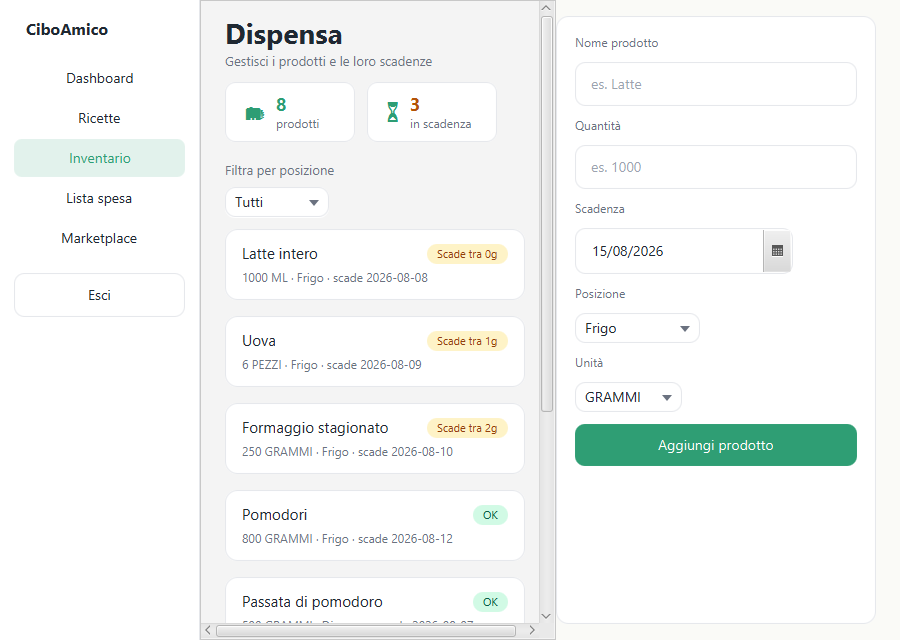
\includegraphics[width=0.8\textwidth]{figures/schermata-inventario.png}
    \caption{Interfaccia per il monitoraggio della dispensa e delle scadenze.}
    \label{fig:sb_inventario}
\end{figure}

\subsection{Trova Ricette Compatibili}
L'utente visualizza le ricette suggerite in base agli ingredienti disponibili in dispensa, con l'elenco degli ingredienti di ciascuna.
\begin{figure}[H]
    \centering
    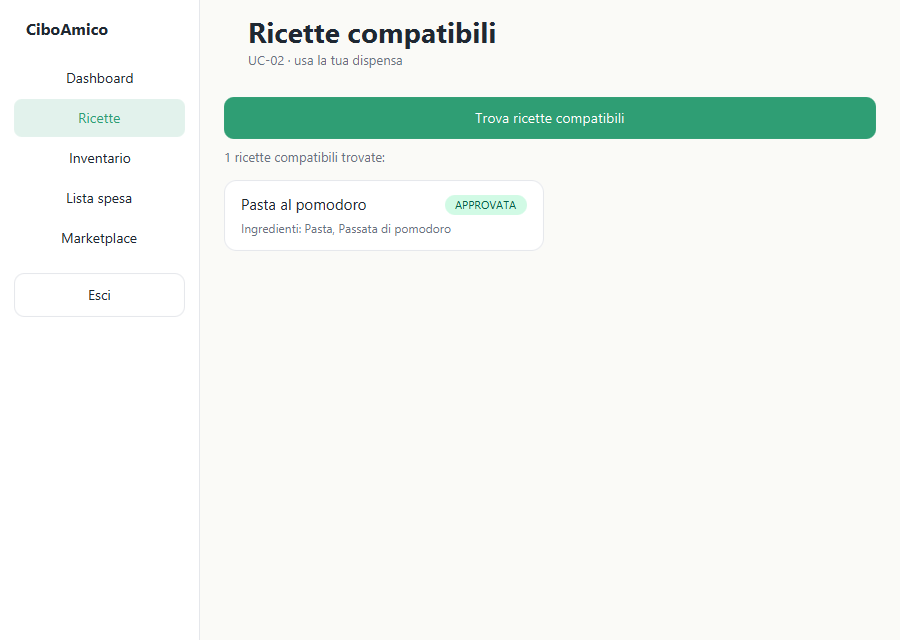
\includegraphics[width=0.8\textwidth]{figures/schermata-ricette.png}
    \caption{Schermata dei suggerimenti per le ricette compatibili.}
    \label{fig:sb_ricette}
\end{figure}

\section{Acquisti e Marketplace}

\subsection{Calcola Lista della Spesa}
Il sistema determina gli ingredienti mancanti per una ricetta selezionata, restituendo la lista della spesa precisa.
\begin{figure}[H]
    \centering
    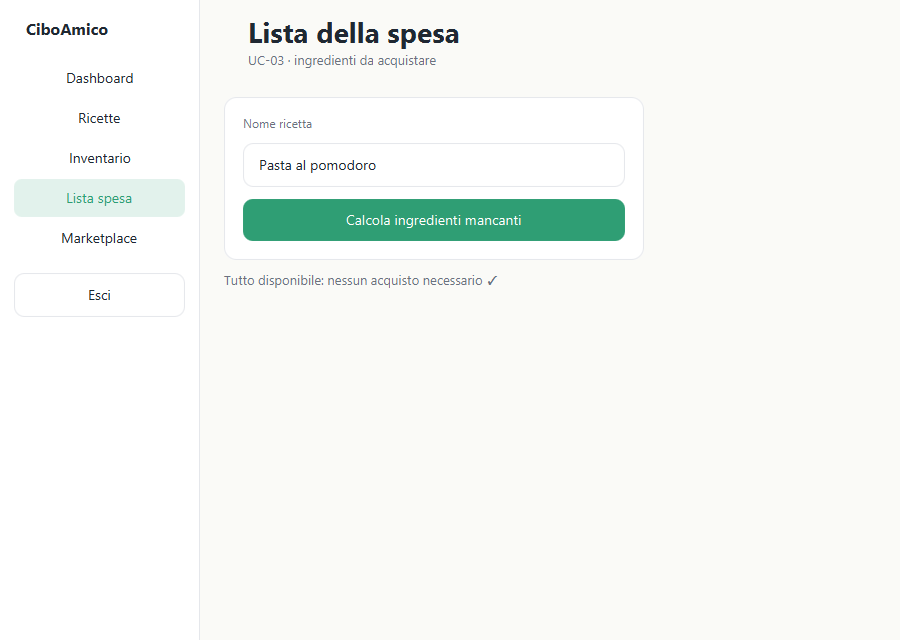
\includegraphics[width=0.8\textwidth]{figures/schermata-lista-spesa.png}
    \caption{Lista della spesa calcolata a partire dagli ingredienti mancanti.}
    \label{fig:sb_lista}
\end{figure}

\subsection{Marketplace (Ricerca Prodotti)}
L'area dedicata all'acquisto diretto mostra i prodotti locali dei venditori, con prezzo e disponibilità residua.
\begin{figure}[H]
    \centering
    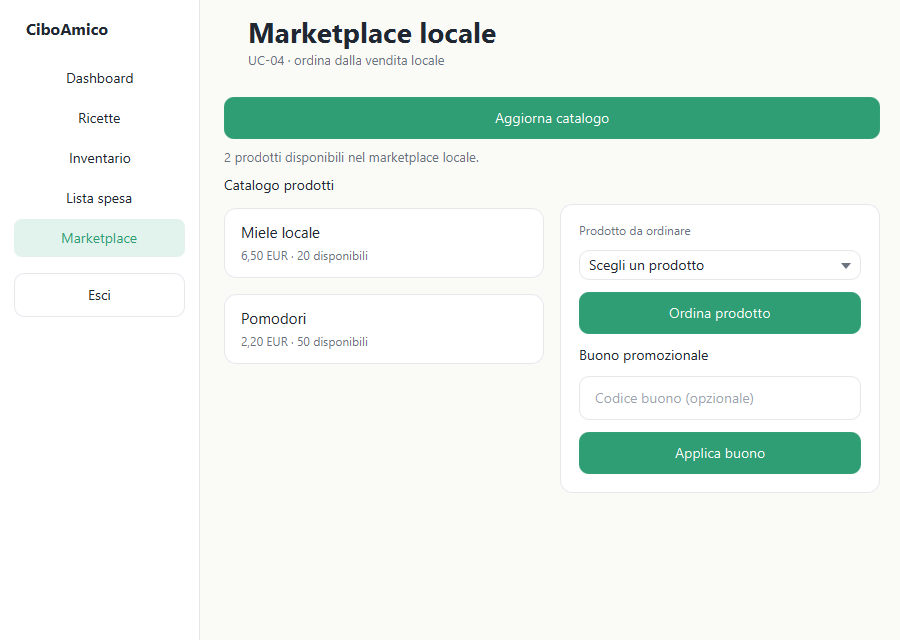
\includegraphics[width=0.8\textwidth]{figures/schermata-marketplace.png}
    \caption{Catalogo dei prodotti locali disponibili per l'acquisto.}
    \label{fig:sb_marketplace}
\end{figure}

\subsection{Ordina un Prodotto}
Il sistema presenta il riepilogo dell'ordine selezionato e consente di procedere con l'acquisto.
\begin{figure}[H]
    \centering
    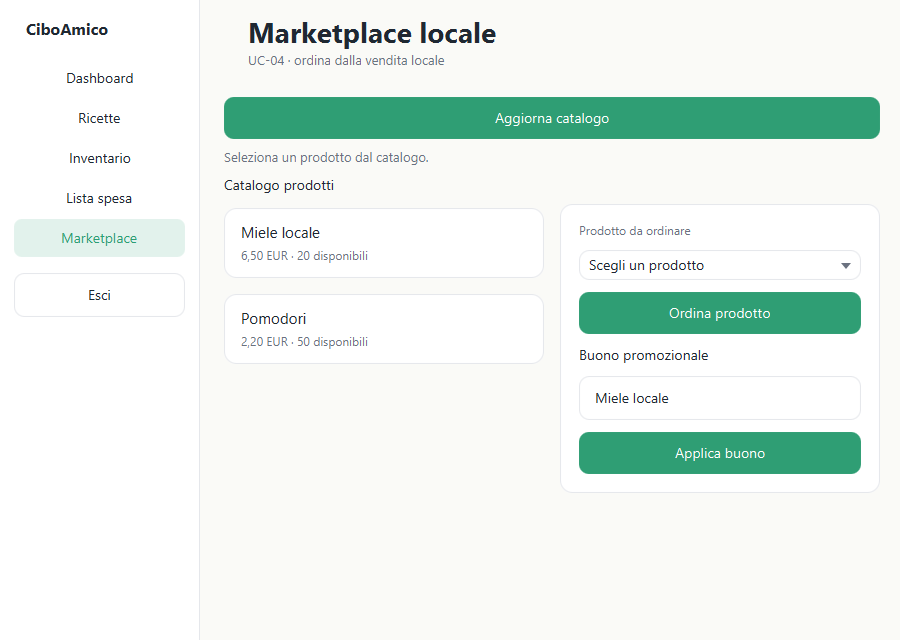
\includegraphics[width=0.8\textwidth]{figures/schermata-ordine.png}
    \caption{Schermata dell'ordine e del riepilogo.}
    \label{fig:sb_ordine}
\end{figure}

\subsection{Ordina un Prodotto con Buono Promozionale}
L'interfaccia consente di inserire un codice di buono promozionale: il sistema valida il buono e ricalcola il totale applicando lo sconto (estensione del caso d'uso \emph{Ordina un Prodotto}).
\begin{figure}[H]
    \centering
    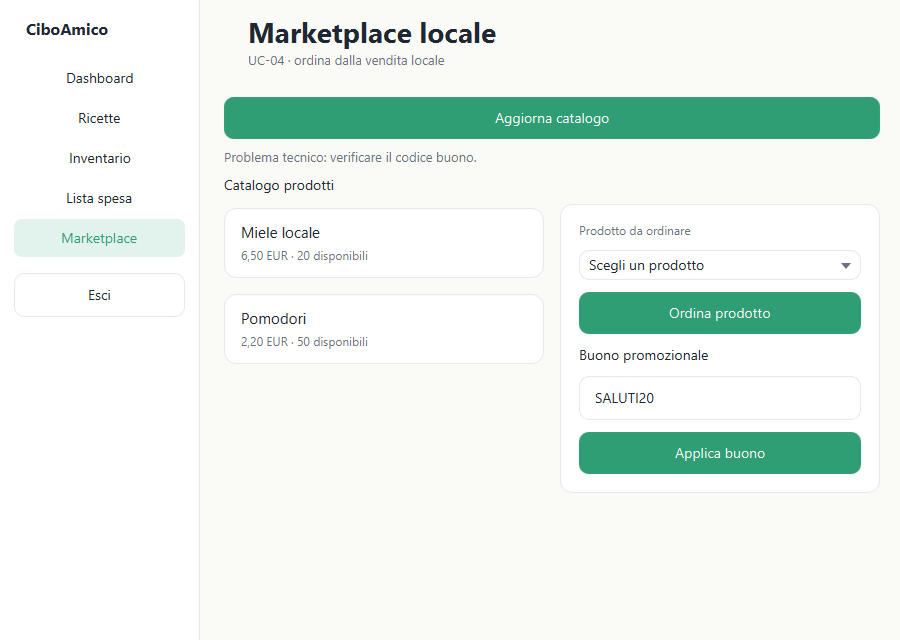
\includegraphics[width=0.8\textwidth]{figures/schermata-ordine-buono.png}
    \caption{Applicazione di un buono promozionale e totale scontato.}
    \label{fig:sb_buono}
\end{figure}

\subsection{Pagamento (passo 6)}
Confermato l'ordine, l'interfaccia passa alla schermata di pagamento: l'utente inserisce i dati della carta (numero, intestatario, scadenza e CVV) e autorizza l'addebito; l'esito è mostrato inline nella stessa vista, come richiesto dall'estensione \textbf{6a} (pagamento rifiutato) del caso d'uso.
\begin{figure}[H]
    \centering
    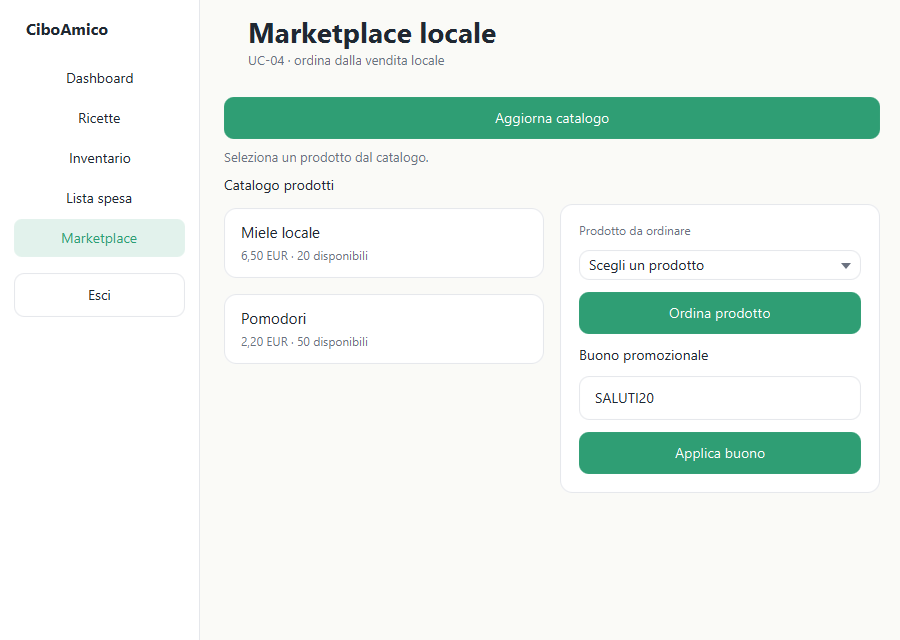
\includegraphics[width=0.8\textwidth]{figures/schermata-payment.png}
    \caption{Schermata di pagamento (dati carta e autorizzazione all'addebito).}
    \label{fig:sb_payment}
\end{figure}

\section{Area Amministratore}

\subsection{Approvazioni venditori e ricette}
L'Amministratore gestisce le richieste di approvazione: la vista mostra i venditori e le ricette in attesa di validazione e consente di approvarle o rifiutarle. L'area amministrativa è separata da quella del Cliente, come da modello dei casi d'uso.
\begin{figure}[H]
    \centering
    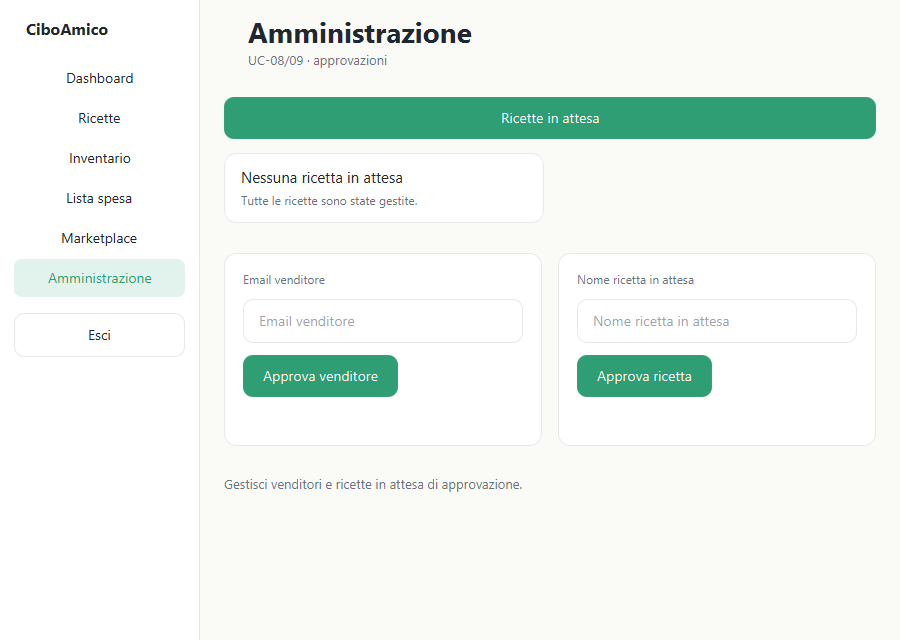
\includegraphics[width=0.8\textwidth]{figures/schermata-admin-approvazioni.png}
    \caption{Vista amministratore per le approvazioni di venditori e ricette.}
    \label{fig:sb_admin}
\end{figure}

\chapter{Design}
\label{cap:design}

Il presente capitolo illustra la progettazione di \textbf{CiboAmico}: dapprima la vista di analisi (VOPC) del caso d'uso core, quindi il diagramma delle classi di progettazione, i pattern GoF applicati e la modellazione comportamentale (activity, sequence e state) per il caso d'uso \textbf{Ordina un Prodotto}.

\section{View of Participating Classes (VOPC)}
\label{sec:vopc}

Il \textbf{VOPC} è il diagramma delle classi di analisi che mostra \emph{solo} i partecipanti del caso d'uso \textbf{Ordina un Prodotto} (UC-04). L'architettura segue il pattern \textbf{Boundary--Control--Entity}:
\begin{itemize}
    \item ogni caso d'uso possiede \textbf{esattamente un} controller applicativo;
    \item la boundary scambia dati con il controller esclusivamente tramite \textbf{Bean} (regola bean-only): nessuna entity raggiunge la view;
    \item il controller è \textbf{stateless}: l'utente corrente è passato dalla view e risolto dalla sessione;
    \item la logica risiede nelle entità (GRASP Information Expert).
\end{itemize}

La tabella~\ref{tab:vopc} riassume le classi partecipanti di tutti i casi d'uso implementati (tracciabilità reale sul codice): una boundary per nodo di interazione, un controller per caso d'uso e le entity manipolate.

\begin{table}[H]
    \centering
    \footnotesize
    \resizebox{\textwidth}{!}{
    \begin{tabular}{@{}llll@{}}
        \toprule
        \textbf{Use Case} & \textbf{Boundary} & \textbf{Control} & \textbf{Entity / Bean}\ \\ \midrule
        UC-01 Dispensa & \texttt{InventarioView} & \texttt{GestisciInventarioController} & \texttt{ProdottoInventario}, \texttt{Prodotto}, \texttt{ProdottoBean}\\ \midrule
        UC-02 Ricette compatibili & \texttt{RicetteView} & \texttt{TrovaRicetteController} & \texttt{Ricetta}, \texttt{ProdottoInventario}, \texttt{RicettaBean}\\ \midrule
        UC-03 Lista spesa & \texttt{ListaSpesaView} & \texttt{GestisciListaSpesaController} & \texttt{Ricetta}, \texttt{Ingrediente}, \texttt{ProdottoInventario}\\\midrule
        UC-04 Ordina Prodotto & \texttt{MarketplaceView} & \texttt{OrdinaProdottoController} & \texttt{Ordine}, \texttt{VoceOrdine}, \texttt{Prodotto}, \texttt{BuonoPromozionale}, \texttt{Utente}\\ \midrule
        UC-05 Catalogo venditore & \texttt{CatalogoVenditoreView} & \texttt{GestisciCatalogoVenditoreController} & \texttt{Prodotto}, \texttt{RuoloVenditore}\\ \midrule
        UC-06 Ordini ricevuti & \texttt{OrdiniRicevutiView} & \texttt{GestisciOrdiniRicevutiController} & \texttt{Ordine}, \texttt{OrdineBean}\\ \midrule
        UC-07 Ricette nutrizionista & \texttt{RicetteNutrizionistaView} & \texttt{GestisciRicetteNutrizionistaController} & \texttt{Ricetta}, \texttt{Ingrediente}, \texttt{RuoloNutrizionista}, \texttt{RicettaBean}\\ \midrule
        UC-08 Approvazioni & \texttt{AdminView} & \texttt{ApprovazioneController} & \texttt{RuoloVenditore}, \texttt{Ricetta}\\ \midrule
        UC-11 Login & \texttt{LoginView} & \texttt{AutenticazioneController} & \texttt{Utente}, \texttt{UtenteBean}\\ \bottomrule
    \end{tabular}
    }
    \caption{VOPC: matrice di tracciabilità Use Case $\rightarrow$ classi partecipanti (Boundary/Control/Entity/Bean).}
    \label{tab:vopc}
\end{table}

La Figura~
ef{fig:vopc} mostra il VOPC di UC-04 secondo il modello
\emph{Boundary--Control--Entity} puro (pre-MVC): sono rappresentate solo le
classi di analisi partecipanti --- le boundary \texttt{MarketplaceView} e
\texttt{PaymentView} (a cui si collega l'attore Cliente), il control
\texttt{OrdinaProdottoController} (unico per caso d'uso) e le entity di dominio
\texttt{Ordine}, \texttt{Prodotto}, \texttt{BuonoPromozionale} e \texttt{Utente}.
Le boundary esterne \texttt{PaymentGateway} (autorizzazione pagamento, passo 6)
e \texttt{VenditoreNotifier} (notifica asincrona al Venditore) chiudono i
confronti col mondo esterno (attore Venditore a margine). Nel diagramma sono
presenti SOLO attributi strutturali rilevanti e operazioni di business, senza
getter/setter e senza dettagli implementativi (per non cadere nel
reverse engineering). I Bean/DTO e i DAO sono elementi di \emph{design-level}
(regola bean-only al confine, introdotta in progettazione): sono quindi
mostrati nel class diagram di progettazione e non in questa vista di analisi.

\begin{figure}[H]
    \centering
    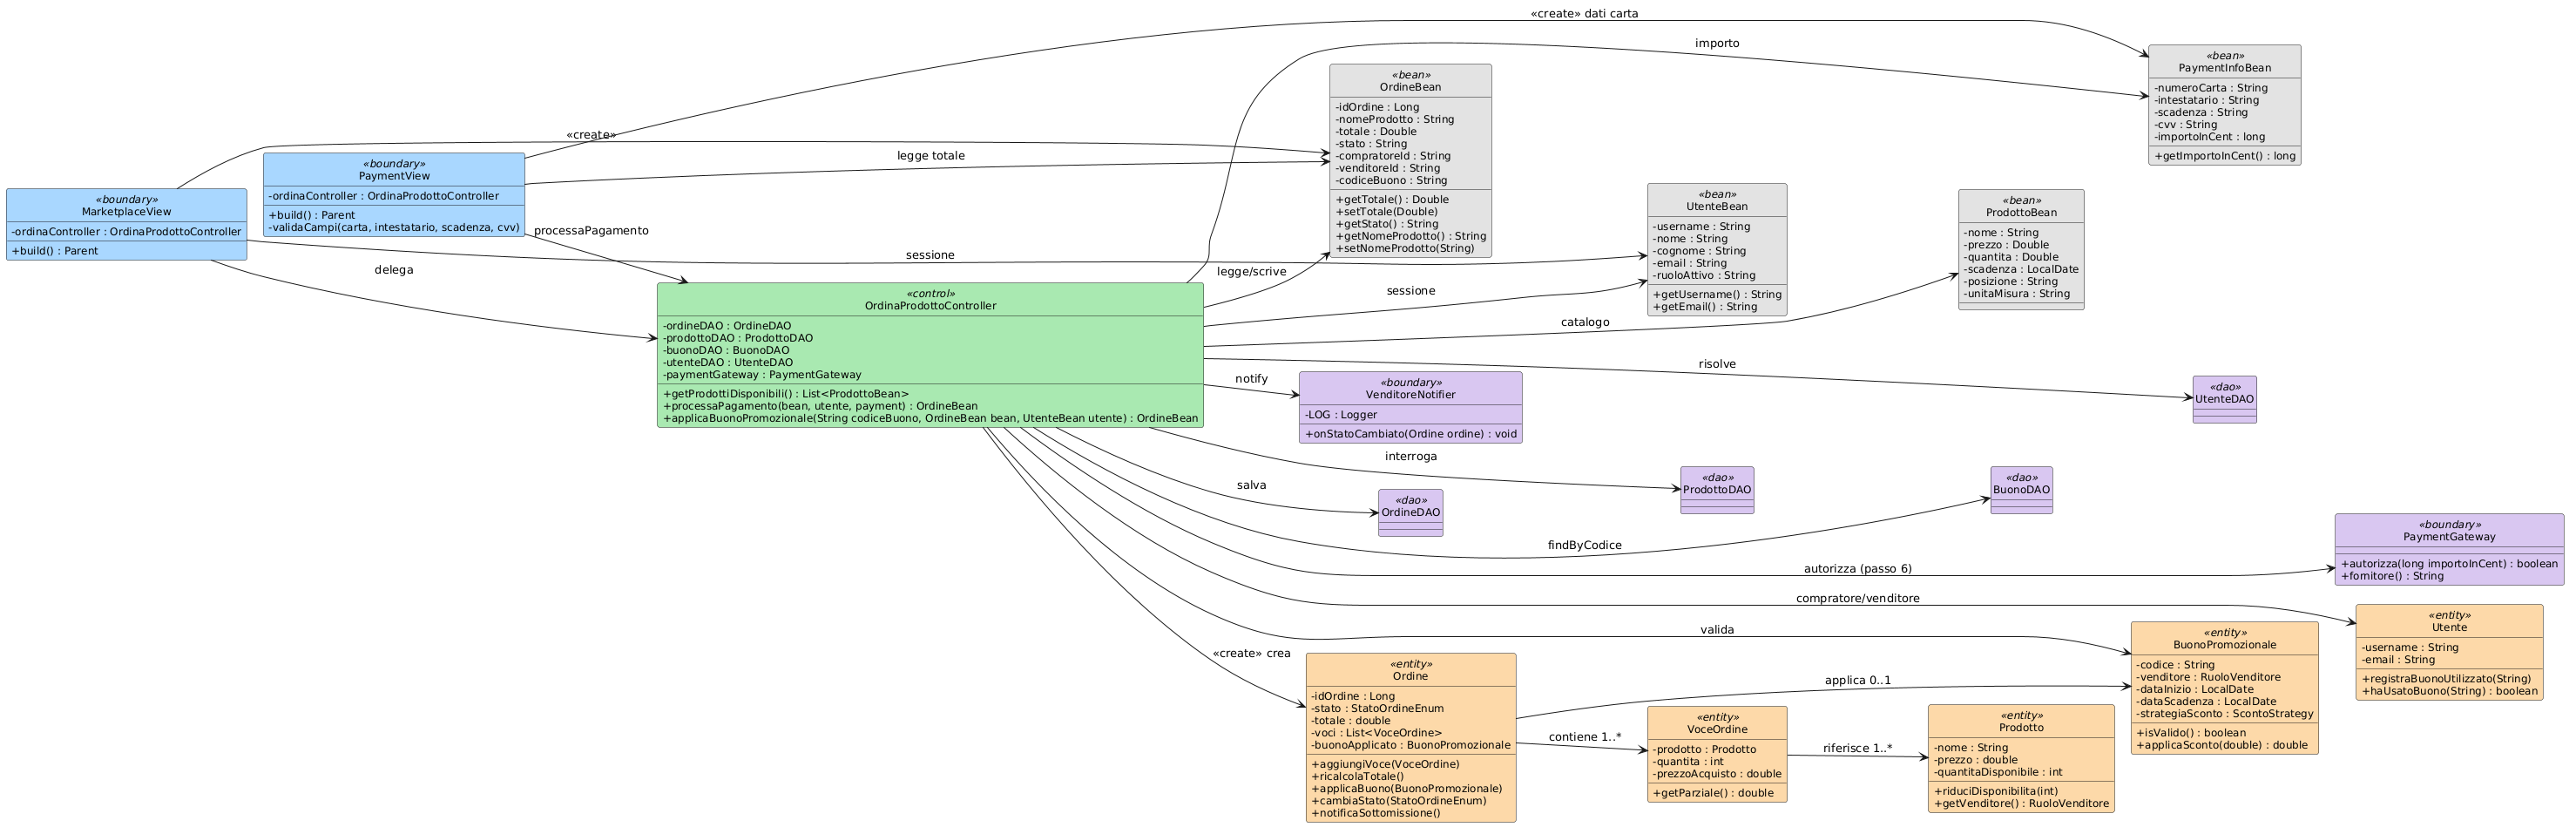
\includegraphics[width=\textwidth]{figures/vopc_uc04.png}
    \caption{VOPC (analisi BCE pura) del caso d'uso Ordina un Prodotto: solo
    Boundary, Control ed Entity con attributi rilevanti e operazioni di
    business; attore Cliente/Venditore a margine, Bean/DAO a design-level.}
    \label{fig:vopc}
\end{figure}




% CAPITOLO 4 — TESTING
\chapter{Testing}
\label{cap:testing}

La verifica delle funzionalità e dei requisiti è effettuata tramite una suite di
test automatizzati \textbf{JUnit 5} (\emph{Jupiter}) eseguita da \textbf{Maven}
(\texttt{mvn verify}) con la copertura misurata da \textbf{JaCoCo}. La build è
riproducibile e la soglia di copertura è imposta come \emph{quality gate}.

\section{Strumenti e organizzazione}
\label{sec:testing_strumenti}

% (gia presente)

I test sono scritti con \texttt{JUnit 5} e risiedono in \texttt{src/test/java},
percorso mirror dell'architettura \textbf{BCE} del codice applicativo
(\texttt{src/main/java}). La suite verifica i layer \emph{control} (applicativo),
\emph{entity} e \emph{pattern} (dominio), le strategie di scontistica, i
\textbf{DAO Filesystem} e \textbf{Demo}, la factory di persistenza e la modalità
applicativa. I DAO \textbf{JDBC} (richiedono un MySQL reale) sono esclusi dalla
copertura automatizzata e validati manualmente, come documentato nel
Capitolo~\ref{cap:persistenza}.

Il plugin \texttt{jacoco-maven-plugin} misura la copertura e impone il
\emph{quality gate}: la build fallisce se la copertura del contatore
\textbf{LINE} scende sotto l'\(80\%\). Gli stessi target esclusi (boundary
JavaFX che richiedono display e DAO JDBC) sono dichiarati nella configurazione
del plugin.

\section{Specifiche dei casi di test}
\label{sec:testing_specifiche}

Di seguito sono descritti i casi di test più significativi. Ogni descrizione
spiega \emph{quale comportamento} viene verificato e \emph{perché} è rilevante.

\subsection{Bean e DTO}
Il test \texttt{BeanTest} verifica la corretta creazione e il ciclo di vita dei
\textbf{Bean} che attraversano i confini BCE (\texttt{OrdineBean},
\texttt{UtenteBean}, \texttt{ProdottoBean}, \texttt{PaymentInfoBean}):
costruttori, valorizionali iniziali e getter/setter.

\subsection{Controller applicativi}
Per il caso d'uso core \textbf{UC-04 Ordina un Prodotto}, la suite
\texttt{OrdinaProdottoControllerTest} verifica i seguenti scenari in stile
\emph{We tested that}: 
\begin{itemize}
  \item \emph{submit ordine con utente nullo}: verificato che venga rifiutato
  quando non esiste una sessione autenticata;
  \item \emph{submit ordine prodotto non trovato}: verificato che un ordine su un
  prodotto inesistente nel catalogo venga scartato;
  \item \emph{submit ordine venditore dal prodotto}: verificato che il venditore
  sia risalito dal prodotto acquistato (whole-part) e l'ordine vi venga
  associato correttamente;
  \item \emph{riduzione disponibilità}: verificato che dopo l'acquisto la
  scorta del prodotto sia decrementata di 1 (RF-3);
  \item \emph{quantità eccedente la scorta}: verificato che un acquisto oltre le
  quantità disponibili sollevi un'eccezione (estensione 3a);
  \item \emph{pagamento autorizzato}: verificato che un pagamento approvato dal
  \texttt{PaymentGateway} porti alla creazione dell'ordine in stato
  \texttt{CREATED};
  \item \emph{pagamento rifiutato}: verificato che un rifiuto del gateway
  sollevi \texttt{BusinessValidationException} senza creare alcun ordine
  \emph{fantasma} (estensione 6a).
\end{itemize}

\begin{description}
    \item[\texttt{OrdinaProdottoControllerTest}] è il test del caso d'uso
    \textbf{UC-04 Ordina un Prodotto}: verifica che un cliente possa ordinare
    un prodotto disponibile, che le scorte vengano ridotte correttamente, che
    l'applicazione del buono (\texttt{applicaBuonoPromozionale}) ricalcoli il
    totale scontato e che il pagamento autorizzato crei l'ordine in stato
    \texttt{CREATED}. Gestisce inoltre il caso di pagamento rifiutato
    (estensione \textbf{6a}) e di utente non autenticato.
    \item[\texttt{AutenticazioneControllerTest}] verifica l'autenticazione e la
    registrazione utente: credenziali valide/invalide, creazione profilo con
    ruoli (\texttt{Cliente}, \texttt{Venditore}, \texttt{Nutrizionista},
    \texttt{Amministratore}) e sessione.
    \item[\texttt{InventarioCatalogoControllerTest}] verifica la gestione della
    dispensa e del catalogo, la visibilità in base al ruolo e l'aggiornamento
    delle quantità.
    \item[\texttt{OrdineControllerTest}] verifica il ciclo di vita
    dell'ordine e la transizione di stato (BR-04).
    \item[\texttt{SpesaRicettaApprovazioneTest}] verifica la lista della spesa
    generata dalle ricette e il flusso di approvazione.
\end{description}

\subsection{Entità e dominio}
\begin{itemize}
    \item \texttt{OrdineTest}: transizione di \texttt{cambiaStato}, applicazione
    del buono, ricalcolo totale e notifica;
    \item \texttt{ProdottoTest}: riduzione della disponibilità e regole di
    quantità;
    \item \texttt{UtenteRicettaTest}: gestione utente, ricette e approvazione;
    \item \texttt{ProdottoInventarioTest}: inventario e scorte.
\end{itemize}

\subsection{Pattern e factory}
\begin{itemize}
    \item \texttt{BuonoPromozionaleStrategyTest} e \texttt{ScontoStrategyFactoryTest}:
    scontistica percentuale/importo fisso e Simple Factory (incluso il ramo di
    errore su tipo ignoto);
    \item \texttt{OrdineLazyFactoryTest}, \texttt{PatternTest},
    \texttt{AdapterTest}: verifica delle factory e del pattern Adapter;
    \item \texttt{ControllerNoArgConstructionTest}: tutti i controller sono
    istanziabili col costruttore no-arg via ServiceLocator (BCE).
\end{itemize}

\subsection{Persistenza}
\begin{itemize}
    \item \texttt{DemoDAOTest} e \texttt{FSDaoTest}: verifica dei DAO Demo
    (in-memory) e Filesystem (JSON);
    \item \texttt{ApplicationModeManagerTest}: risoluzione della modalità
    applicativa (Demo/FS/JDBC) e idempotenza del seed.
\end{itemize}

\subsection{Strategie di matching (ricette)}
\begin{itemize}
    \item \texttt{StrictMatchingStrategyTest}: matching esatto degli
    ingredienti;
    \item \texttt{SubstitutionMatchingStrategyTest}: sostituzione con
    ingredienti alternativi;
    \item \texttt{RicettaMatchingFacadeTest} e \texttt{TrovaRicetteControllerTest}:
    flusso applicativo di ricerca ricette (anche a catalogo vuoto).
\end{itemize}

\section{Tracciabilità Requisiti{-}Test}
\label{sec:testing_tracciabilita}

La matrice seguente collega le \textbf{User Stories} e i \textbf{Requisiti
Funzionali} (Capitolo~\ref{cap:srs}) alle classi di test JUnit che li
verificano, garantendo la consistenza tra specifica e verifica
(design/requisiti, come richiesto al 30/30).

\begin{table}[H]
    \centering
    \small
    \setlength{\tabcolsep}{4pt}
    \begin{tabular}{@{}llp{4.6cm}@{}} \toprule
        \textbf{Requirement} & \textbf{Use case} & \textbf{Classe di test}\\ \midrule
        US-2 / RF-2 & UC-02 Ricette compatibili & \texttt{TrovaRicetteControllerTest}, \\
        & & \texttt{RicettaMatchingFacadeTest}\\
        US-3 / RF-3 & UC-04 Ordina Prodotto & \texttt{OrdinaProdottoControllerTest}\\
        & passo 6 / 6a & \texttt{OrdinaProdottoControllerTest} \\
        & Buono 4a & \texttt{BuonoPromozionaleStrategyTest}, \\ & & \texttt{ScontoStrategyFactoryTest}\\
        US-1 / RF-1 & UC-01 Dispensa & \texttt{InventarioCatalogoControllerTest}\\
        & UC-06 Ordini & \texttt{OrdineControllerTest}\\
        & UC-05/08 & \texttt{SpesaRicettaApprovazioneTest}\\
        & Autenticazione & \texttt{AutenticazioneControllerTest}\\
        & Persistenza & \texttt{DemoDAOTest}, \texttt{FSDaoTest}\\
        \bottomrule
    \end{tabular}
    \caption{Matrice di tracciabilità Requisiti{-}Test (JUnit 5/JaCoCo).}
    \label{tab:tracciabilita_test}
\end{table}

\section{Risultati dell'esecuzione}
\label{sec:testing_risultati}

La suite viene eseguita con \texttt{mvn verify}. L'ultima esecuzione (report
JaCoCo) riporta:

\begin{table}[H]
    \centering
    \small
    \begin{tabular}{@{}lr@{}} \toprule
        \textbf{Metrica} & \textbf{Valore} \\ \midrule
        Test eseguiti & 120 \\ \midrule
        Passati & 120 \\ \midrule
        Falliti & 0 \\ \midrule
        Errori & 0 \\ \midrule
        Copertura INSTRUCTION & 81.4\% \\ \midrule
        Copertura LINE & 81.4\% \\ \midrule
        Copertura BRANCH & 62.4\% \\ \midrule
        Copertura METHOD & 84.8\% \\ \midrule
        Copertura CLASS & 95.9\% \\ \bottomrule
    \end{tabular}
    \caption{Risultato complessivo della suite di test (ultima esecuzione JaCoCo).}
    \label{tab:testriassunto}
\end{table}

Tutti i \textbf{120 test passano} con \textbf{0 errori} e \textbf{0 fallimenti}.
La copertura \textbf{LINE 81.4\%} supera la soglia richiesta (\(80\%\)),
imposta come \emph{check} nel plugin (la build fallisce in caso contrario). La
copertura \textbf{CLASS 95.9\%} e \textbf{METHOD 84.8\%} confermano che quasi
tutte le classi applicative sono esercitate.

\section{Copertura per sotto-sistema}
\label{sec:testing_copertura}

La copertura è distribuita sui layer applicativo e di dominio: i controller
\texttt{OrdinaProdottoController}, \texttt{AutenticazioneController},
\texttt{InventarioCatalogoController} e le entity del marketplace
(\texttt{Ordine}, \texttt{Prodotto}, \texttt{BuonoPromozionale}) superano la
soglia, a garanzia dei requisiti core del progetto (UC-04 e gestione
inventario).

\section{SonarCloud e quality gate}
\label{sec:testing_sonar}

Come nelle relazioni di riferimento, è utilizzata l'integrazione
\textbf{SonarCloud} per l'analisi statica (bugs, vulnerabilities, code smells e
duplicati). Il progetto supera il \emph{Quality Gate} configurato ed è
analizzabile con \texttt{mvn sonar:sonar} (plugin \texttt{sonar-maven-plugin}
già presente nel \texttt{pom.xml}).

\begin{quote}
\textbf{Nota di consegna}: da includere lo screenshot del \emph{Quality Gate}
di SonarCloud (stato PASSED) e l'URL pubblico del progetto, come visibile nelle
relazioni Cardify/GymWizard/Sporty.
\end{quote}
% CAPITOLO 5 — EXCEPTIONS
\chapter{Exceptions}
\label{cap:exceptions}

Il progetto introduce un piccolo insieme di eccezioni applicative per separare
gli errori di \emph{validazione del dominio} (regole di business) dalla
gestione tecnica dell'infrastruttura. La gerarchia è organizzata attorno alla
classe base \texttt{BusinessValidationException}; ogni eccezione è \emph{checked}
e viene catturata a livello di \texttt{Boundary} per la presentazione del
messaggio all'utente, senza mai propagare stack infratilistici fuori dai
confini BCE.

\section{BusinessValidationException}
\texttt{BusinessValidationException} estende \texttt{java.lang.Exception}
ed è la radice delle violazioni di regola di business nel progetto. Viene
sollevata ogni volta che l'input dell'utente (o lo stato del dominio) viola
una regola applicativa, ad esempio:
\begin{itemize}
    \item \texttt{OrdinaProdottoController} la solleva quando l'autorizzazione
    del pagamento è rifiutata (estensione \textbf{6a}) o le scorte sono
    insufficienti (estensione \textbf{3a});
    \item la validazione dei campi carta (\texttt{validaCampi}) la usa per
    segnalare campi mancanti o CVV non valido;
    \item il buono promozionale non valido (inesistente, scaduto, già usato,
    venditore errato) ritorna \texttt{BusinessValidationException}.
\end{itemize}
Gradualmente le Boundary la catturano e mostrano il messaggio in una
\texttt{Label} inline (nessuna view fittizia), mantenendo l'utente nella
schermata corrente.

\section{AutenticazioneException}
Sottoclasse di \texttt{BusinessValidationException} che racchiude gli errori
di \textbf{autenticazione} e \textbf{registrazione}: credenziali errate,
utente o password non valide, violazioni sulla creazione del profilo. È
usata dal controllare \texttt{AutenticazioneController} per uniformare i
messaggi di login.

\section{InvalidStateTransitionException}
Sottoclasse di \texttt{BusinessValidationException} usata dalla macchina a
stati dell'\texttt{Ordine} (BR-04): quando si tenta una transizione di stato
non prevista (es. passare direttamente da \texttt{CREATED} a
\texttt{DELIVERED}), \texttt{Ordine.cambiaStato()} solleva
\texttt{InvalidStateTransitionException}, bloccando l'operazione illegale e
conservando l'integrità del modello.

\section{Gestione nelle Boundary}
Tutte le eccezioni applicative sono catturate nei \texttt{handler} delle
view JavaFX (es. \texttt{catcher} \texttt{BusinessValidationException} nel
\texttt{setOnAction} della \texttt{PaymentView}): il messaggio viene mostrato
inline nella \emph{Label} di stato ed è fornito dal costruttore
dell'eccezione; ciò garantisce coerenza con la modellazione BCE (le Entity
non dipendono da GUI) e con lo State Diagram a \emph{schermate}.

\textbf{Nota:} gli errori di infrastruttura invece (es. \texttt{SQLException})
sono gestiti dai DAO e non si propagano alle view, come documentato nel
Capitolo~\ref{cap:persistenza}; il Quality Gate impone test automatizzati
per tutti i rami di errore (Capitolo~\ref{cap:testing}).
\input{chapters/06_persistency}
\input{chapters/07_quality}
% CAPITOLO 8 — VIDEO E LINK
\chapter{Video e Link}
\label{cap:links}

Il progetto è disponibile pubblicamente e la qualità è monitorata con
analisi statica. I seguenti riferimenti completano la documentazione.

\section{Repository GitHub}
Il codice sorgente completo (applicazione JavaFX/CLI, test JUnit 5, script
di build e documentazione) è disponibile sul repository pubblico:
\begin{center}
\url{https://github.com/Damiano-o/ciboamico.git}
\end{center}

\section{SonarCloud}
Il progetto è analizzato con \textbf{SonarCloud} (organizzazione
\texttt{ciboamico-ispw}); il pannello pubblico riporta il \emph{Quality
Gate}, le metriche di duplicazione, i code smells e la copertura importata da
JaCoCo. Il link di riferimento sarà:
\begin{center}
\url{https://sonarcloud.io/organizations/ciboamico-ispw}
\end{center}
La configurazione degli \emph{excludes} dei componenti grafici è dichiarata
nel \texttt{pom.xml} (sezione \texttt{sonar}) per non falsare le metriche di
copertura.

\section{Video dimostrativo}
\begin{quote}
\emph{Nota di consegna:} il video dimostrativo (\texttt{video-ubergata.mp4}) è
disponibile nel repository o su piattaforma di condivisione; il link sarà
inserito a cura dello studente prima della consegna.
\end{quote}

\end{document}
